\section{Power Budget Breakdown}
\label{blBudgetPower}

At this preliminary stage, the power budget breakdown is an estimation based on previous missions and on general data taken from \cite{larson}.

The biggest power requirements come from the mission payload and the power system. The payload needs power to be able to operate the emitter
and the receiver for the whole mission lifetime. About 30$\%$ of the total power will be used to operate the transmitter and 10$\%$ for the receiver. The power distribution and control will take up about 30$\%$ of all the power. Of this 25$\%$ will be needed for the regulators and converters and 5$\%$ will be lost due to wiring losses during the distribution of the power. Furthermore, the \ac{ADCS} system will need approximately 15$\%$ of the total power to be able to operate. The amount of power that will go to its subsystems (sensors, controllers and processors) is an estimate based on previous missions (i.e. FireSat \cite{larson}).

The last subsystem that needs power is Communications. This system is divided further in to the actual communications and the command and data handling subsystem. Each receive about 5$\%$ of the total power. The power distribution for the transmitter and receiver was taken from values of typical X-Band, S-Band and Ku-Band communication subsystems.
For the power distribution of the command and the telemetry unit, average nominal values were used \cite{larson}.

The power breakdown structure and the corresponding power allocation for each system can be seen in figure \ref{fig:powerbudget} on page \pageref{fig:powerbudget}. A tabulated representation of the breakdown estimations can be found in table \ref{epsbudgettable}.

\begin{table} [h]
\centering
\begin{tabular}{p{12cm} | l }
\textbf{SUBSYSTEM} & \textbf{$\%$ OF TOTAL} \\ \hline \hline
\ac{ADCS} & 15  \\
\hspace{1.0cm} Sensor & 3 \\
\hspace{1.0cm} Controllers & 8 \\
\hspace{1.0cm} Processors & 4 \\ 
\ac{CDH} and \ac{TTC} & 10  \\
\hspace{1.0cm} Communications & 5 \\
\hspace{1.0cm} \hspace{1.0cm} Receiver & 1 \\
\hspace{1.0cm} \hspace{1.0cm} Transmitter & 4 \\
\hspace{1.0cm} Data Handling & 5 \\ 
\hspace{1.0cm} \hspace{1.0cm} Command Unit & 1 \\
\hspace{1.0cm} \hspace{1.0cm} Telemetry & 4 \\
Power & 30 \\
\hspace{1.0cm} Regulator/Converters & 25 \\
\hspace{1.0cm} Wiring & 5 \\
Payload & 40\\
\hspace{1.0cm} Emitter & 30 \\
\hspace{1.0cm} Emitter & 10 \\
\end{tabular} 
\caption{Power budget breakdown estimation}
\label{epsbudgettable}
\end{table}

\begin{figure}
\centering
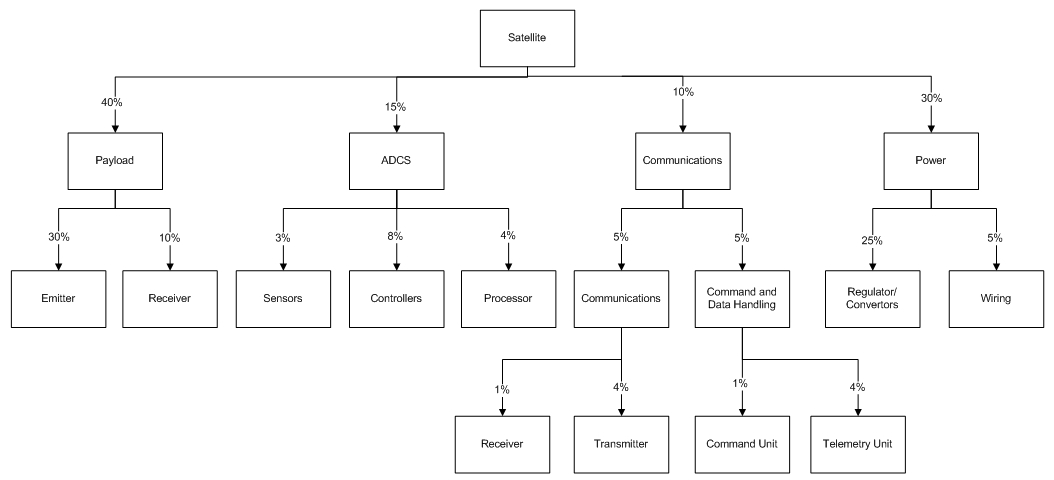
\includegraphics[width=0.9\textwidth, angle=90]{chapters/img/Power_budget_breakdown.jpg}
\caption{Power Budget Breakdown Structure}
\label{fig:powerbudget}
\end{figure}